\documentclass[9pt,twocolumn,twoside]{../../styles/osajnl}
\usepackage{fancyvrb}
\journal{i524} 

\title{Deployment of a Storm cluster}

\author[1,*]{Vasanth Methkupalli}
\author[1,**]{Ajit Balaga}


\affil[1]{School of Informatics and Computing, Bloomington, IN 47408, U.S.A.}

\affil[*]{Corresponding authors:mvasanthiiit@gmail.com}
\affil[**]{Corresponding authors: ajit.balaga@gmail.com}


\dates{project-P015, \today}

\ociscodes{Storm, Ansible, Java, Python}

% replace this with your url in github/gitlab
\doi{\url{https://github.com/cloudmesh/classes/blob/master/project/S17-IR-P015/report/report.pdf}}


\begin{abstract}

Apache Storm is a free and open source distributed realtime
computation system. Storm makes it easy to reliably process unbounded
streams of data, doing for realtime processing what Hadoop did for
batch processing. Storm is simple, can be used with any programming
language. Storm has many use cases: realtime analytics, online machine
learning, continuous computation, distributed RPC etc. Storm is really
fast at data processing: a sample benchmark clocked it at over a
million tuples processed per second per node. It is scalable,
fault-tolerant, guarantees that data will be processed, and is easy to
set up and operate. Storm integrates with the queueing and database
technologies we already use. Storm is currently being used to run
various critical computations in Twitter at scale, and in real-time,
this led us to explore and deploy it on various cloud. In this paper
we try to deploy storm on various clouds and benchmark the performance
on various data, doing real time processing on sample datasets. First,
we describe the architecture of Storm, its deployment and its methods
for distributed scaleout and fault-tolerance. Storm is in active
development at Twitter.
\newline
\end{abstract}

\setboolean{displaycopyright}{true}

\begin{document}

\appendix
\maketitle

\tableofcontents


\section{Introduction}

Currently modern data processing environments require processing
complex computation on streaming data in real-time. Places like
Twitter where each interaction with a user requires making a number of
complex decisions, often based on data that has just been created,
this mandates for a real time data processing system, Storm currently
delivers on this account and provides many other services which we
will see in the coming sections. Storm is designed to be, some of
these things we observed while running our sample projects for
deployment:
\begin{enumerate}
\item Scalable : Nodes may be easily added or removed
  from the Storm cluster without disrupting existing data flows
  through Storm topologies see Fig 3.
\item Resilient : Fault -tolerance is crucial to Storm as it is often
  deployed on large clusters, and hardware components can fail.  The
  Storm cluster must continue processing existing topologies with a
  minimal performance impact.
\item Extensible : Storm topologies may call arbitrary external
  functions (e.g. looking up a MySQL service for the social graph),
  \cite{bronson2013tao} and thus needs a framework that allows
  extensibility.
\item  Efficient : Since Storm is used in
  real-time applications, it must have good performance
  characteristics. Storm uses a number of techniques, including
  keeping all its storage and computational data structures in memory.
\item Easy to Administer : A critical part of storm features or
  development is that it should be easy to administer. Given that
  there a lot of computations going on at every stage, tools should be
  developed which warn the user and development team of any major
  conflicts arising.
\end{enumerate}


\section{Data Model and Architecture}
Storm data processing architecture consists of streams of tuples
flowing through topologies \cite{storm} . A topology is a directed
graph where the vertices represent computation and the edges represent
the data flow between the computation components. Vertices are further
divided into two disjoint sets, spouts and bolts. Spouts are tuple
sources for the topology.  Typical spouts pull data from queues, such
as Kafka \cite{kafka} or Kestrel. On the other hand, bolts process the
incoming tuples and pass them to the next set of bolts downstream.
Note that a Storm topology can have cycles. From the database systems
perspective, one can think of a topology as a directed graph of
operators.
\begin{figure}
  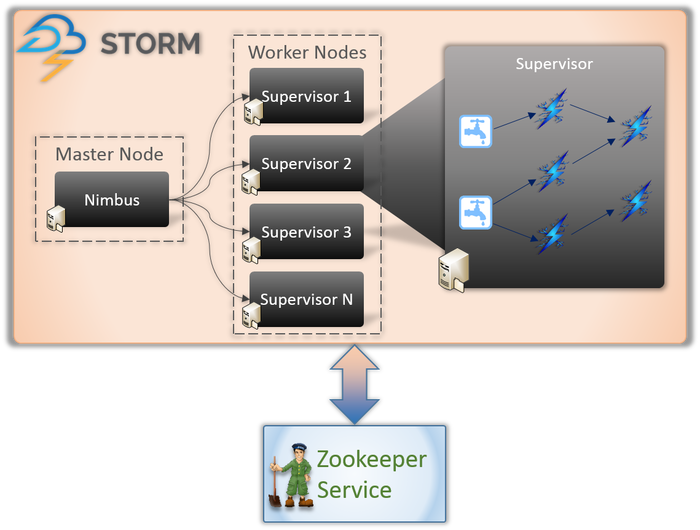
\includegraphics[width=\linewidth]{images/apache-storm.png}
  \caption{Storm Architecture}
  \label{Storm Architecture}
\end{figure}

\subsection{Storm Overview}
Storm runs on a distributed cluster. Clients submit topologies to a
master node, called the Nimbus. The nimbus is responsible for
distributing and coordinating the execution of the topology. The
actual work is done on worker nodes. Each worker node runs one or more
worker processes. At any point in time, a single machine may have more
than one worker processes, but each worker process is mapped to a
single topology. Note more than one worker process on the same machine
may be executing different part of the same topology. Each worker
process runs a JVM, in which it runs one or more executors. Executors
are made of one or more tasks. The actual work for a bolt or a spout
is done in the task. Thus, tasks provide intrabolt or intraspout
parallelism, and the executors provide intratopology
parallelism. Worker processes serve as containers on the host machines
to run Storm topologies. Note that associated with each spout or bolt
is a set of tasks running in a set of executors across machines in a
cluster. Data is shuffled from a producer spout or bolt to a consumer
bolt (both producer and consumer may have multiple tasks). This
shuffling is like the exchange op erator in parallel databases.

Storm supports the following types of partitioning strategies \cite{storm}:

\begin{enumerate}  
\item Shuffle grouping, which randomly partitions the tuples.
\item Fields grouping, which hashes on a subset of the tuple
  attributes or fields.
\item All grouping, which replicates the entire stream to all the
  consumer tasks.
\item Global grouping, which sends the entire stream to a single bolt.
\item Local grouping, which sends tuples to the consumer bolts in the
  same executor.
  
\end{enumerate}
The partitioning strategy is extensible and a topology can define and
use its own partitioning strategy.  Each worker node runs a Supervisor
that communicates with Nimbus.  The cluster state is maintained in
Zookeeper \cite{www-zookeeper}, and Nimbus is responsible for scheduling
the topologies on the worker nodes and monitoring the progress of the
tuples flowing through the topology. Loosely, a topology can be
considered as a logical query plan from a database systems
perspective. As a part of the topology, the programmer specifies how
many instances of each spout and bolt must be spawned. Storm creates
these instances and also creates the interconnections for the data
flow. We note that currently, the programmer has to specify the number
of instances for each spout and bolt. Part of future work is to
automatically pick and dynamically changes this number based on some
higher-level objective, such as a target performance objective.

\subsubsection{Storm Internal Architecture}

In this section, we describe the key components of Storm), and how
these components interact with each other.

\subsubsection{Nimbus and Zookeeper}

Nimbus plays a similar role as the “JobTracker” in Hadoop, and is the
touchpoint between the user and the Storm system. Nimbus is an Apache
Thrift service and Storm topology definitions are Thrift objects.  To
submit a job to the Storm cluster (i.e. to Nimbus), the user describes
the topology as a Thrift object and sends that object to Nimbus. With
this design, any programming language can be used to create a Storm
topology.


As part of submitting the topology, the user also uploads the user
code as a JAR file to Nimbus. Nimbus uses a combination of the local
disk(s) and Zookeeper to store state about the topology. Currently the
user code is stored on the local disk(s) of the Nimbus machine, and
the topology Thrift objects are stored in Zoo keeper.


The Supervisors contact Nimbus with a periodic heartbeat protocol,
this comes in very handy so we can periodically verify ifthe nodes are
working, advertising the topologies that they are currently running,
and any vacancies that are available to run more topologies. Nimbus
keeps track of the topologies that need assignment, and does the match
-making between the pending topologies and the Supervisors.

All coordination between Nimbus and the Supervisors is done using
Zookeeper. Furthermore, Nimbus and the Supervisor daemons are fail-
fast and stateless, and all their state is kept in Zookeeper or on the
local disk(s). This design is the key to Storm’s resilience. If the
Nimbus service fails, then the workers still continue to make forward
progress. In addition, the Supervisors restart the workers if they
fail.

However, if Nimbus is down, then users cannot submit new topologies.
Also, if running topologies experience machine failures, then they
cannot be reassigned to different machines until Nimbus is revived.
An interesting direction for future work is to address these
limitations to make Storm even more resilient and reactive to
failures. All the above workings, whether Nimbus and Zookeeper are
working properly are viewed in the UI of the storm deployment, and can
be viewed from the localhost of that particular node.
\subsubsection{Supervisor}


The supervisor runs on each Storm node. It receives assignments from
Nimbus and spawns workers based on the assignment. It also monitors
the he alth of the workers and respawns them if necessary. The main
thread reads the Storm configuration, initializes the S upervisor’s
global map, creates a persistent local state in the file system, and
schedules recurring timer events. There are three types of events,
which are:

\begin{enumerate}
\item The heart beat event, which is scheduled to run every 15
  seconds, and is runs in the context of the main thread. It reports
  to Nimbus that the supervisor is alive.
\item The synchronize supervisor event, which is executed every 10
  seconds in the event manager thread. This thread is responsible for
  managing the changes in the existing assignments. If the changes
  include addition of new topologies, it downloads the necessary JAR
  files and libraries, and immediately schedules a synchronize process
  event .
\item The synchronize process event, which runs every 3 seconds under
  the context of the process event manager thread. This thread is
  responsib le for managing worker processes that run a fragment of
  the topology on the same node as the supervisor. It reads worker
  heartbeats from the local state and classifies those workers as
  either valid, timed out, not started, or disallowed. A “timed out”
  work er implies that the worker did not provide a heart beat in the
  specified time frame, and is now assumed to be dead. A “not started
  ” worker indicates that it is yet to be started because it belongs
  to a newly submitted topology, or an existing topology who se worker
  is being moved to this supervisor. Finally, a “disallowed ” worker
  means that the worker should not be running either because its
  topology has been killed, or the worker of the topology has been
  moved to another node.
\end{enumerate}



\section{Milestones}

\begin{itemize}
\item Previous Project idea brainstorming
\item Performing Analysis on local VM- April 17th, 2017
\item Deploying Storm and Hadoop on Chameleon Cloud and Jetstream-
  April 20th, 2017
\item Analysis on the distributed cloud environment- April 27th, 2017
\item Benchmarking- April 27th, 2017
\item Final update with report- May 1st, 2017
\end{itemize}


\section{Technologies}




\begin{center}
 \begin{tabular}{||c c||} 
 \hline
 Usage & Technologies Used\\ [0.5ex]
 \hline\hline
 Distributed Computation and Storage:& Storm \\ 
 \hline
 Development: &Python and Java\\
 \hline
 Deployment: &Ansible, Bash Shell script\\
 \hline
 Project Repository: &GitHub \\
 \hline
 Document Preparation: &LaTex\\ [1ex] 
 \hline
\end{tabular}
\end{center}








  
\section{Deployment Automation}
\subsection{Automation with Ansible}
Ansible Playbook is used as the application and configuration
deployment tool. Deploying the hadoop and spark framework into the
cluster environment. Ansible will help push configurations to the
environment automatically based on playbooks written for various
configurations. For this project, we used Ansible to automate the
deployment of storm, zookeeper and other prequisites. The Ansible
script is written such that we can leverage the cloudmesh client
technology to deploy the spark cluster. When creating Zookeeper
cluster we had a communication issue, similar issue was found when
creating a Storm cluster, we resolved this issue by uploading a
secgroup with the details necessary and added it to the cluster.

The Ansible playbook package constitutes the following files.
\begin{itemize}
\item ansible.cfg: This file contains all the configuration
  information necesasary for the storm deployment. In our project we
  refer to the hosts file to look up for the ips necessary for
  deployment.
  
\item hosts: Efforts are made to automate the generation of this file,
  however currently the user after creating a cluster in the cloudmesh
  client has to update the information the user ip addresses and id's
  in three columns, chameleon, nimbus and supervisors fields. This
  enables the user to select the ip address in which they desire to
  have the nimbus node and all other configuration.

\item install.yml: However, the above step is one of the few steps we
  had to configure manually, however, running the command
  ansible-playbook install.yml, installs all the dependencies and
  packages necessary for strom deployment. However, the install sets
  up the cluster with supervisor and nimbus nodes. The startup of
  these services however are to be done manually by the below bash
  scripts.

\item nimbus.sh: This script is intended to start the nimbus node to
  receive all the packets(data) for processing.
\item startStorm.sh: This starts the storm cluster.
\item submit.sh Used to submit jobs to run, in the storm cluster.
\item start-zookeeper.yml: This file is still in developmental stage
  where we want to automate the above two steps, however, there is a
  small problem in exiting the storm cluster after once it has
  started. We are working on it to fix this.
\item supervisor.sh: This script file is used to start the worker
  nodes on which the data processing can run
\item ui.sh: Running this script file will open the localhost, where
  we can view the current jobs running, topologies, cluster
  information, spouts, bolts, etc. Sample screenshots showing the
  working of this are shown in the benchmarking figures.
\item In the templates folder, we have hosts.j2, myid.j2,
  storm.yaml.j2, zoo.cfg.j2, these files are necessary for proper
  deployment of storm and zookeeper cluster, so we created templates
  of the configuration files and intend to use them.
\end{itemize}  



\subsection{Bash Shell Script}

First we automated the entire deployment using python shell script,
and later changed the deployment by using Ansible playbooks. In the
python shell script, we have mainly used 4 files(.sh) to automate the
entire process, from updating the apps directory to configuring the
host file in the zookeeper cluster. As a part of our project we are
submitting even the python shell script files for everyone to view the
initial stages of project development.
  
\section{Cloudmesh}
Cloudmesh client is a simple client to enable access to multiple cloud
environments form a command shell and commandline[reference for
  cloudmesh].The entire application is built on python which
essentially needs no prerequisite knowledge and hence could see this
as a ready-to-use tool. For our project since we need access to clouds
for deployment purposes this comes as a welcome tool to ease us with
the entire deployment process. Many thanks to Gregor von Laszewski and
others collaborators for supporting our project directly and
indirectly in the form of this tool which enabled us to deploy the
project easier without any hassles. For this project, have tested the
installation on Ubuntu 16.04.

\section{Cloud Deployment}


We selected two clouds for deployment our project: Chameleon Cloud,
and Jetstream. In our automated deployment and benchmarking process,
first we create a cluster of particular number of required nodes,
update the ip addresses and the user id of all the clouds, then we run
the ansible script to deploy the entire project on the cloud. However,
lot of improvements can be made, such as automating the process of ip
addresses for the cluster deployment and exiting the cloud by deleting
the files and the cloud resources once deployed and benchmarked. The
entire process of deploying the project on various clouds have been
tried and tested, various times were measure on the context of
installation time right from the beginning. Based on the above results
we benchmarked our results on various cluster sizes.

\section{Benchmarking}
\subsection{Chameleon Cloud}
Following are the results of our benchmarking on deploying the storm
cluster on Chameleon cloud. Few things, we noticed that a 3-node
cluster is not viable for running storm jobs and hence we ran all our
jobs on 5-nodes or above clusters, this was one error we came across
when we tried deploying a 3-node cluster and overcame this by
following code blogs related to troubleshooting mentioned in the code
references and solved the issue. We ran a sample-storm job on a 5node
cluster to see if its working, following are the snapshots where in we
can see the UI of storm, showing all the resources used among many
other things. Similar tests were made on a 7-node and a 9-node cluster
and results were stored in a log page.



\begin{table}[htbp]
\centering
\caption{\bf Hardware Specifications of Chameleon}

 \begin{tabular} {| c | c |}
\hline
  & Chameleon   \\ [0.5ex] 
 \hline

    
CPU   & Xeon X5550  \\
 \hline
cores & 1008   \\
 \hline
speed & 2.3GHz \\
 \hline
RAM   & 5376GB  \\
 \hline
storage & 1.5PB  \\ [1ex] 
 \hline

\end{tabular}
  \label{tab:cloud-comparison}
\end{table}

\begin{figure}[!htb]
  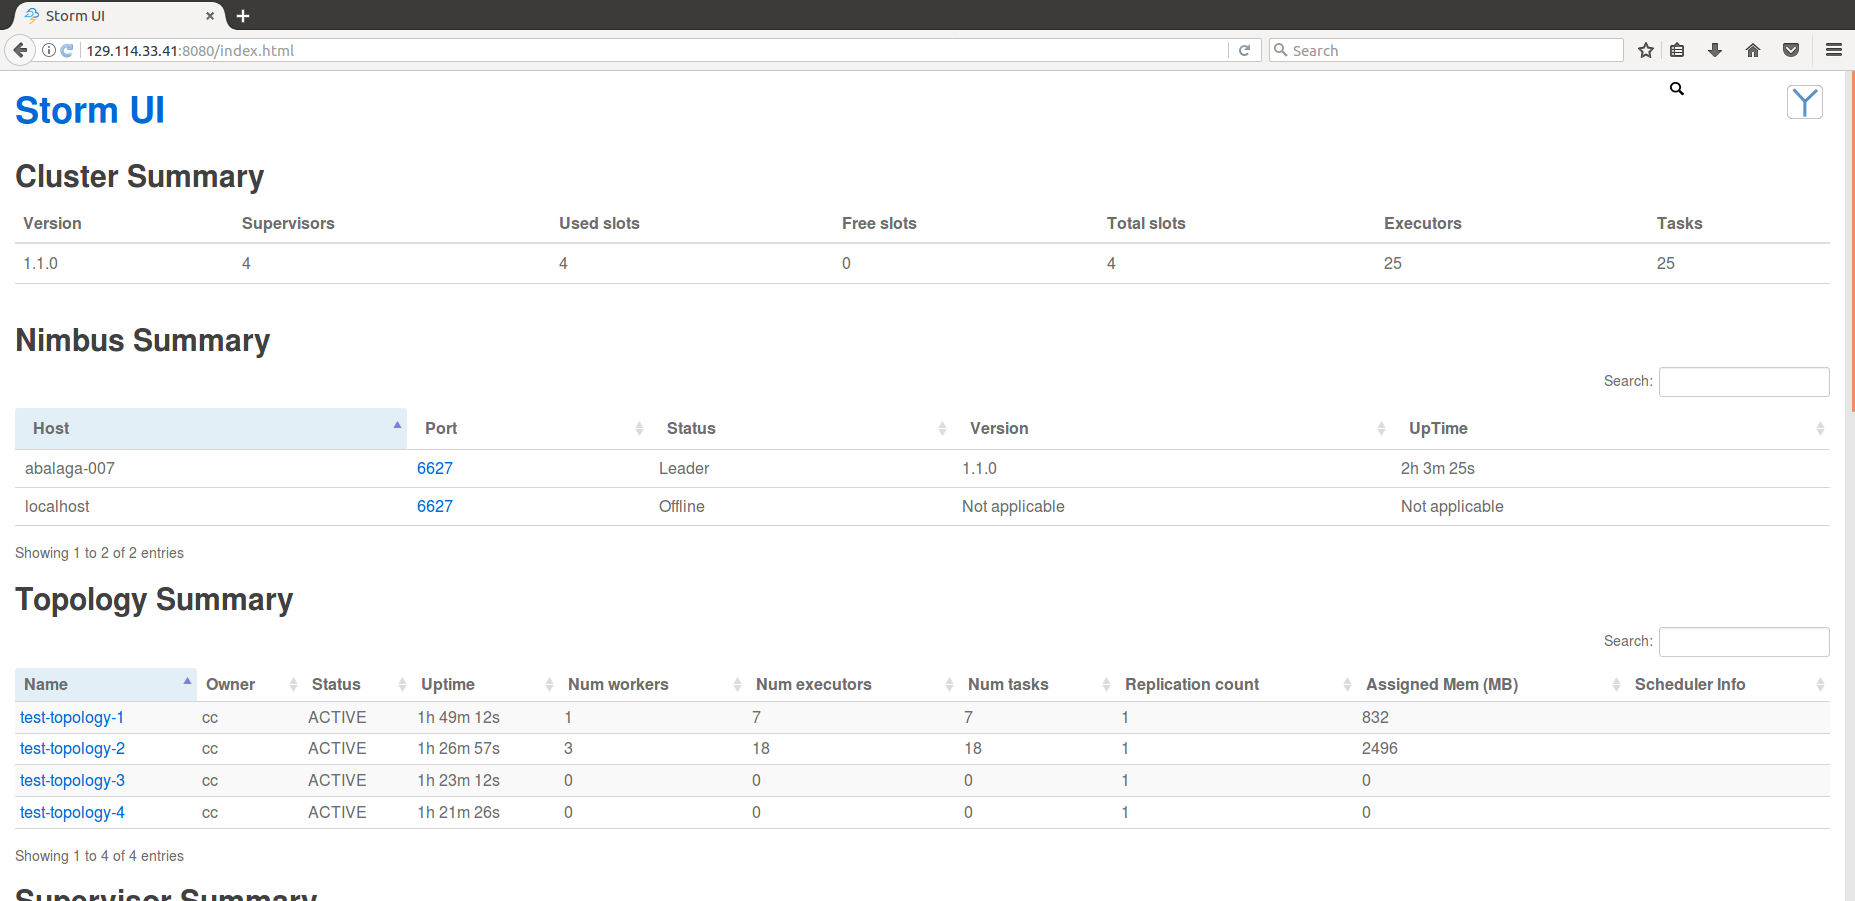
\includegraphics[width=\linewidth]{images/bench-1.png}
  \caption{Index Page}
  \label{Index Page}
\end{figure}


\begin{figure}[!htb]
  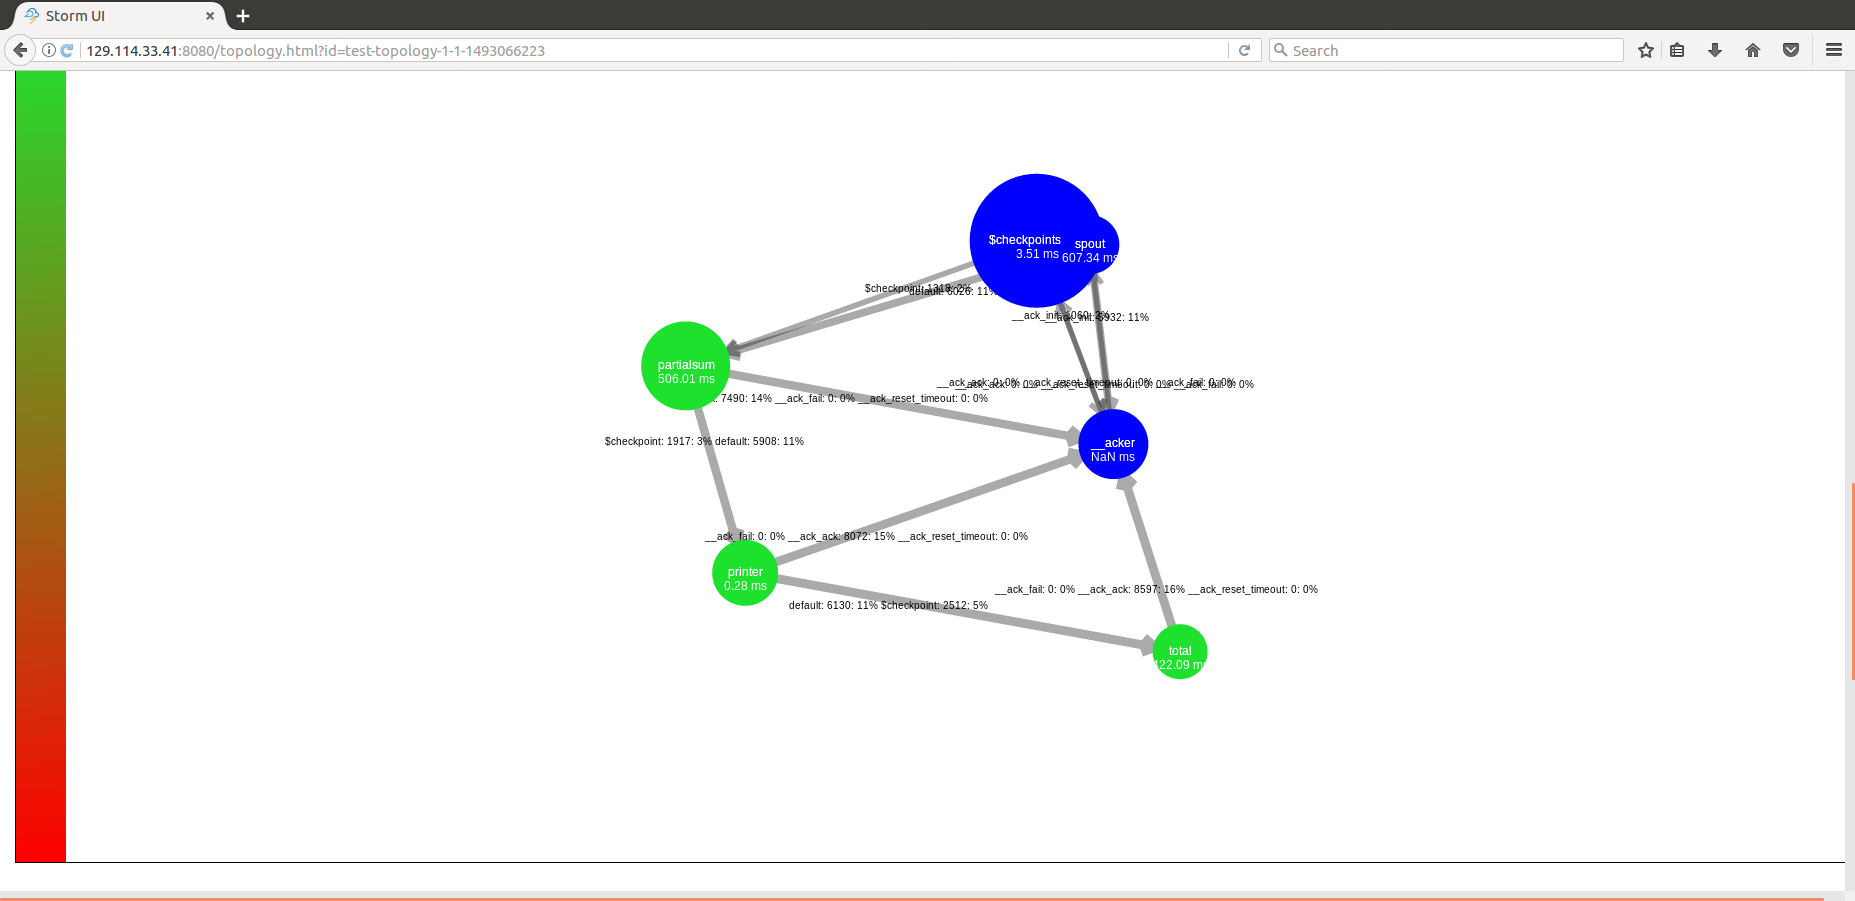
\includegraphics[width=\linewidth]{images/bench-2.png}
  \caption{Sample Topology on a 5-node cluster }
  \label{Sample Topology on a 5-node cluster}
\end{figure}

\begin{figure}[!htb]
  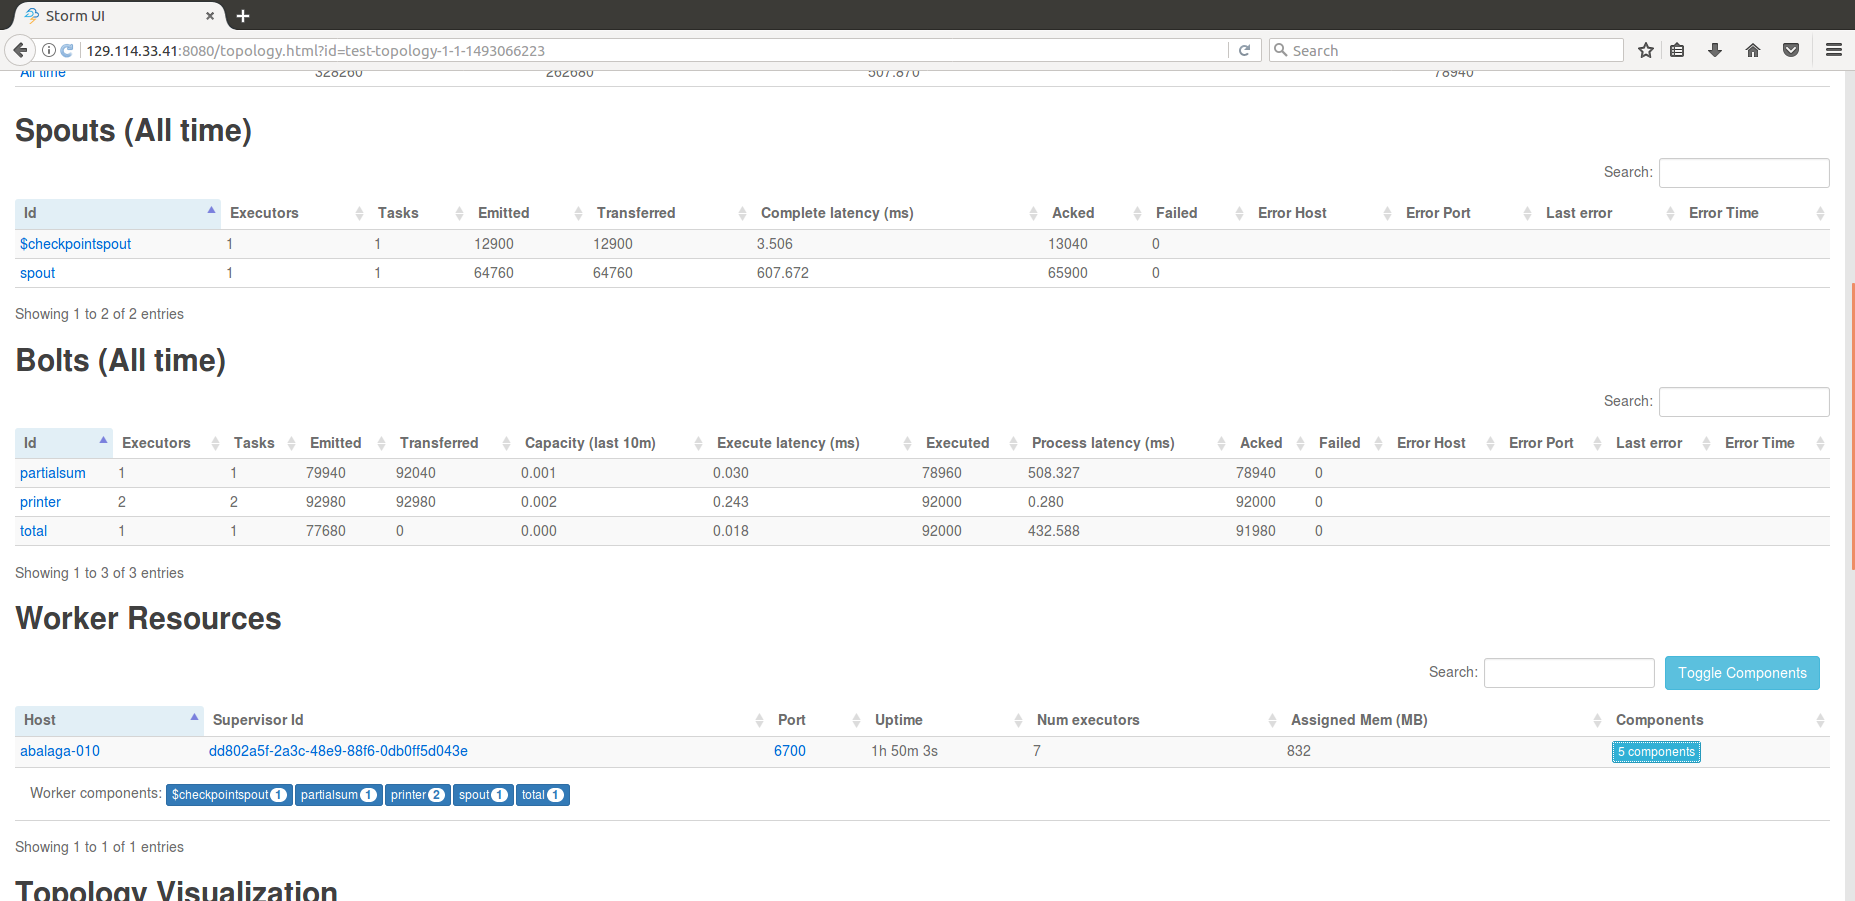
\includegraphics[width=\linewidth]{images/bench-3.png}
  \caption{Worker nodes and description on a 5-node cluster }
  \label{Worker nodes and description on a 5-node cluster}
\end{figure}

\begin{figure}[!htb]
  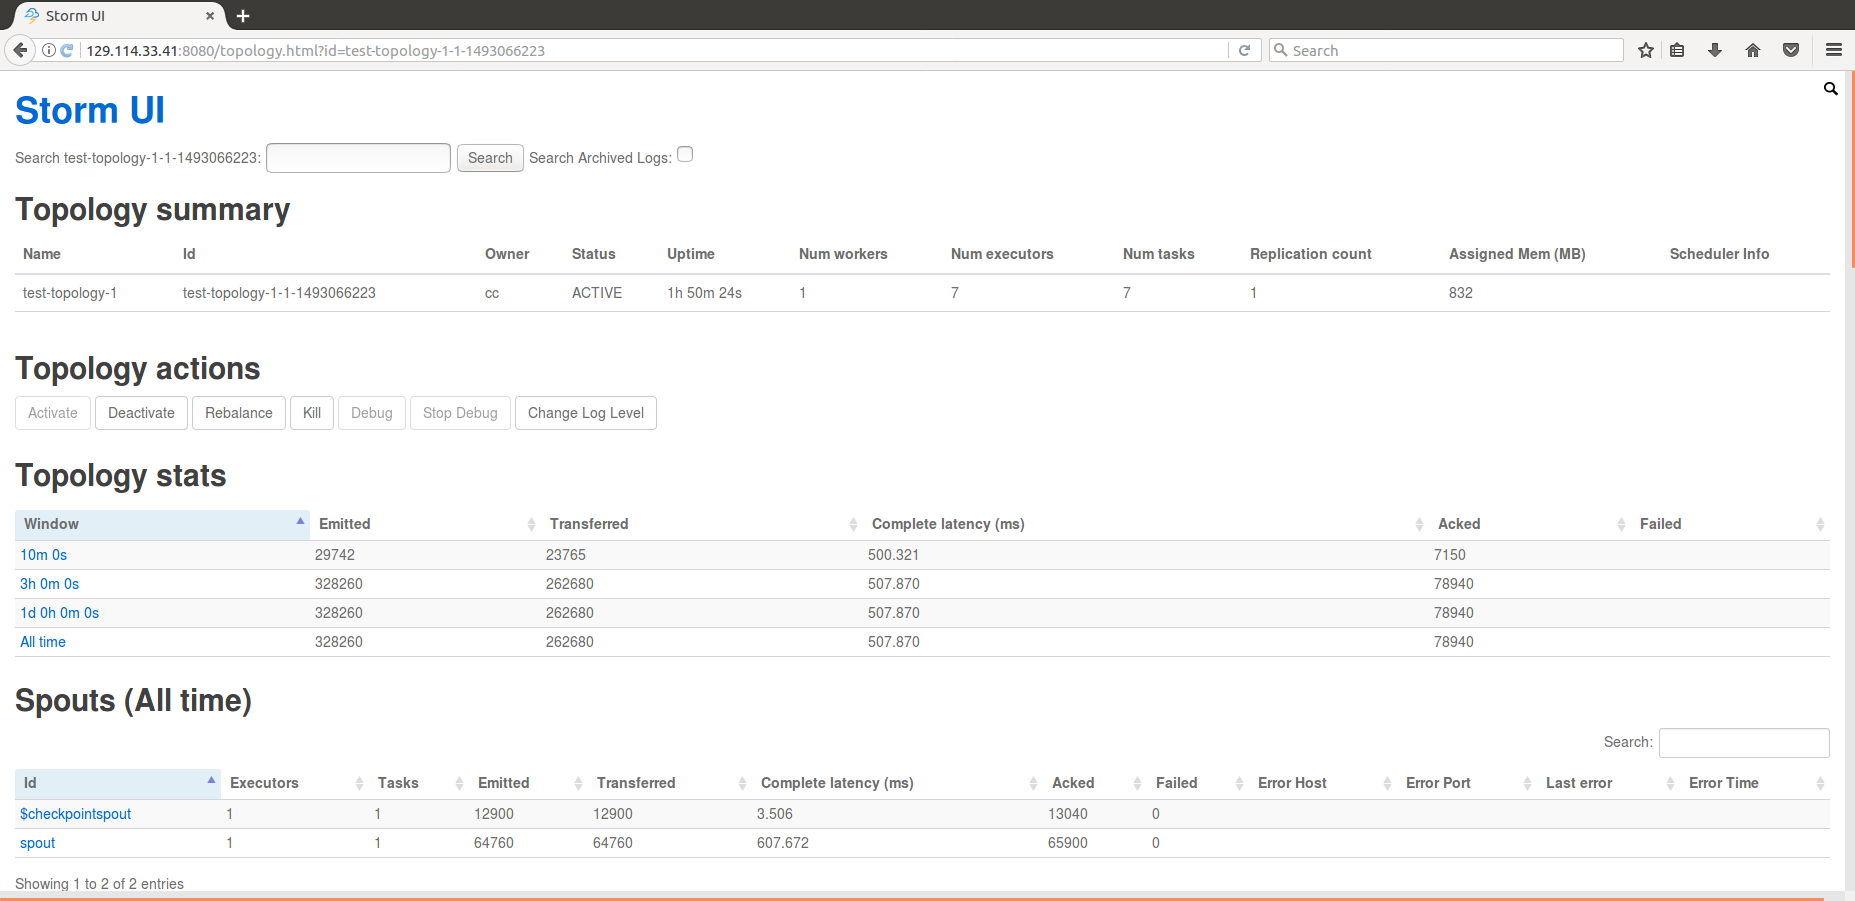
\includegraphics[width=\linewidth]{images/bench-4.png}
  \caption{Toplogy Summer on a 5-node cluster }
  \label{Topology summary on a 5-node cluster}
\end{figure}

\begin{figure}[!htb]
  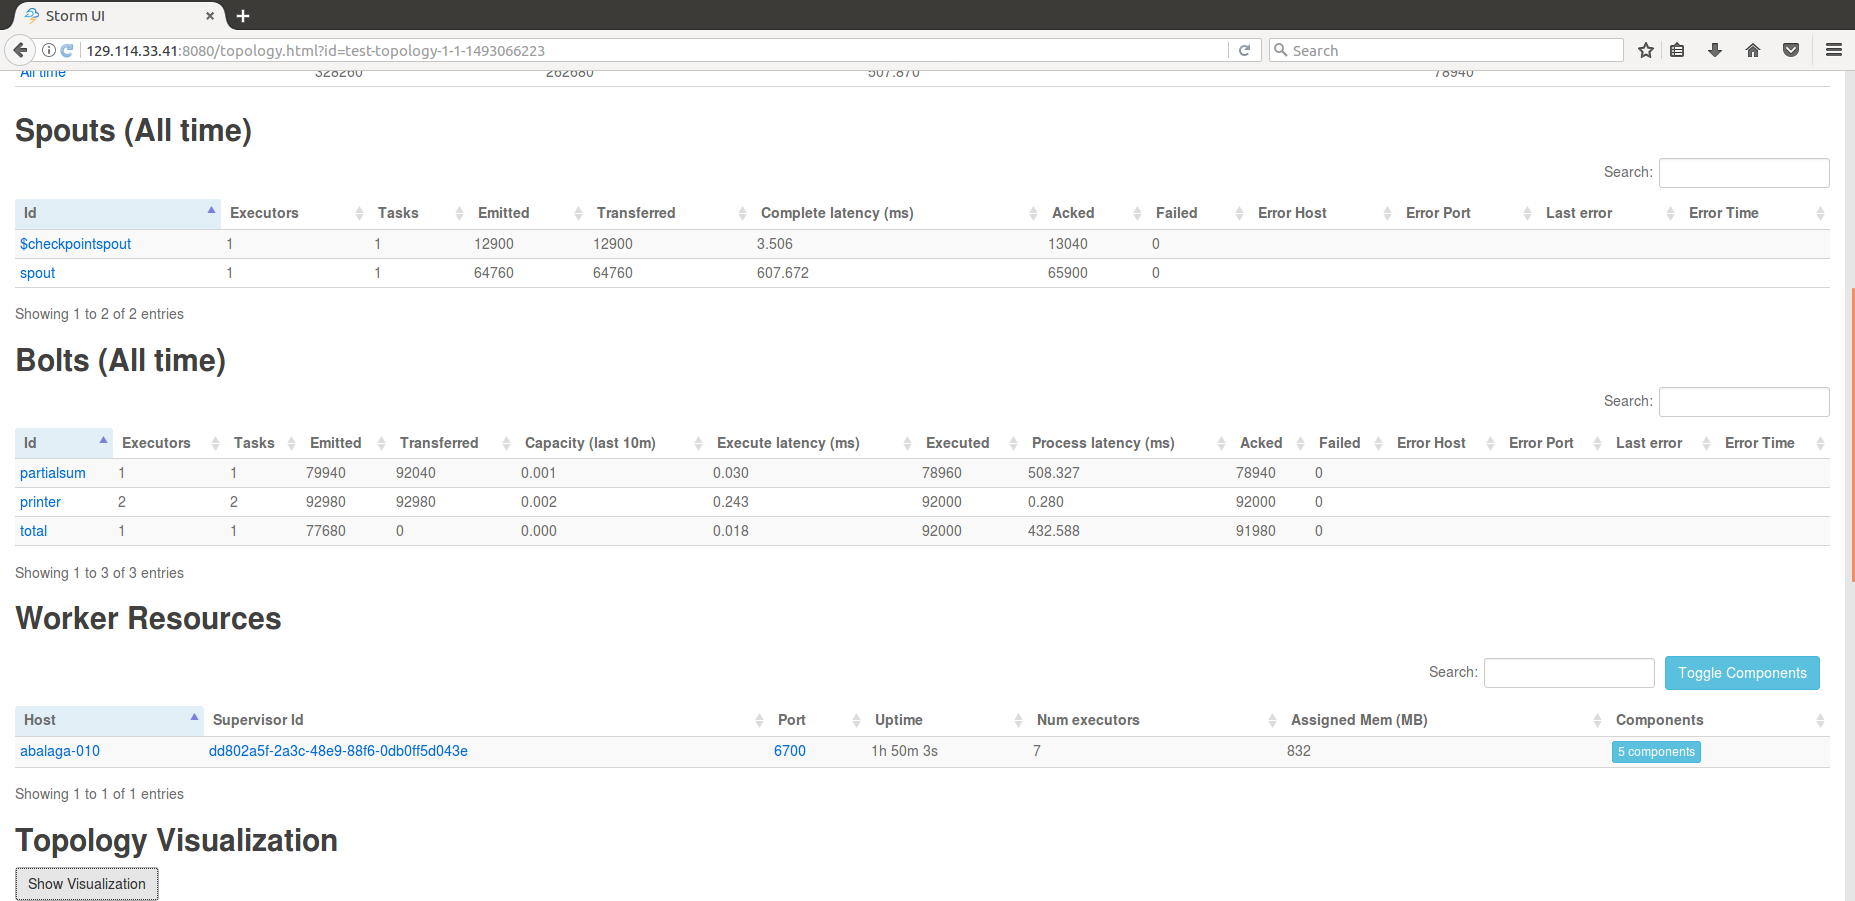
\includegraphics[width=\linewidth]{images/bench-5.png}
  \caption{Spouts and bolts summary on a 5-node cluster }
  \label{Spouts and bolts summary on a 5-node cluster}
\end{figure}



Also we calculated the time it took to deploy a 5-node, 7-node and a 9-node cluster on the chameleon cloud. Following are the results obtained and can be illustrated below.


\begin{figure}[!htb]
  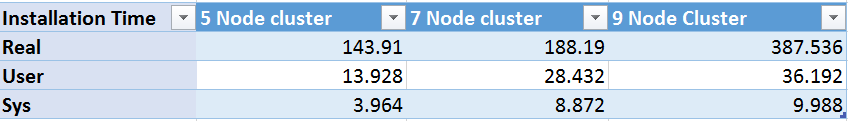
\includegraphics[width=\linewidth]{images/table-1.png}
  \caption{Table showing the time taken to deploy }
  \label{Table showing the time taken to deploy}
\end{figure}


\begin{figure}[!htb]
  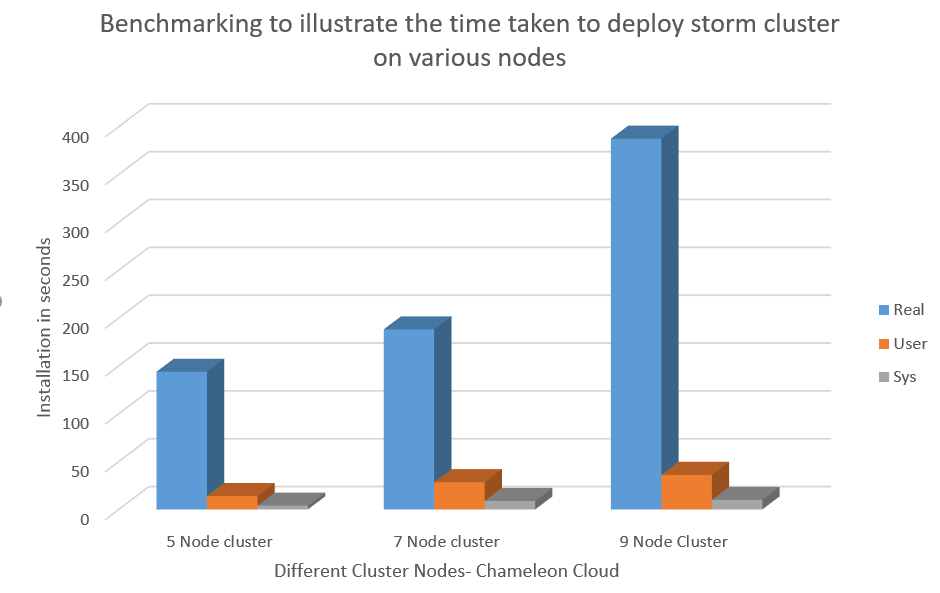
\includegraphics[width=\linewidth]{images/bar-1.png}
  \caption{Bar diagram to compare the time taken to deploy }
  \label{Bar diagram to compare the time taken to deploy}
\end{figure}

\subsection{JetStream}

We had slight issues booting the Virtual Machines on the jetstream
cloud. In that scenario we decided to go ahead and deploy the cluster
only on the chameleon cloud and test its performance. However, it can
be noted that the deployment is fairly similar even in the case of
JetStream using the Cloudmesh client.

\section{Code References}
Following were the code resources used in deploying the cluster at various
stages.
\begin{itemize}
\item
  Storm-\cite{www-storm1}\cite{www-storm2}\cite{www-storm3}\cite{www-storm4}\cite{www-storm5}\cite{www-storm6}\cite{www-storm7}\cite{www-storm8}\cite{www-storm9}\cite{www-storm10}
\item
  Zookeeper-\cite{www-zk1}\cite{www-zk2}\cite{www-zk3}\cite{www-zk4}\cite{www-zk5}\cite{www-zk6}\cite{www-zk7}\cite{www-zk8}
\item Running Topologies on a
  cluster-\cite{www-rtc1}\cite{www-rtc2}\cite{www-rtc3}\cite{www-rtc4}\cite{www-rtc5}\cite{www-rtc6}
\item Zookeeper
  Troubleshooting-\cite{www-zt1}\cite{www-zt2}\cite{www-zt3}\cite{www-zt4}\cite{www-zt5}\cite{www-zt6}
\item Storm Troubleshooting-\cite{www-nnf1}\cite{www-nnf2}\cite{www-nnf3}\cite{www-nnf4}
\item Storm defaults yaml-\cite{www-sd1}
\end{itemize}


\section{Summary}

We have created, tested and demonstrated a fully automated program to
configure and deploy a Storm cluster which can be deployed on cloud
environments. We currently deployed it on Chameleon cloud and expect
to do the same with any other cloud environment with slight changes in
the ansible script.Also, another thing we observed while deploying a
Zookeeper cluster that installing it in standalone mode makes it prone
to breakdown, since if the Zookeeper cluster fails in this scenario,
the entire storm cluster fails to run, however installing it on server
mode leads to the scenario where in if one or more clusters fail to
run, the load is handled by the other nodes in the cluster. We used a
combination of Python, bash, cloudmesh client and ansible in fully
deploying the cluster. We did a benchmark test on Chameleon cloud to
measure the time taken to deploy 5, 7 and 9 node clusters, so far it
has shown satisfactory results and we are striving to take it beyond
to other cloud environments as well.

\section{Acknowledgments}
This project was a part of the Big Data Software and Projects
(INFO-I524) course. We would like to thank Professor Gregor von
Laszewski and the associate instructors for their help and support
during the course. Special mention to cloudmesh client which made most
of the gruelling taks straighforward.


\bibliography{references}
\begin{enumerate}
\section{Work Breakdown}

\item Ajit Balaga: Responsible for initial deplopyment of storm cluster on various clouds and clusters of different sizes, played an instrumental role in understanding the storm toplogy and its architecture. Also, responsible for finding out that a storm cluster is better deployed on a 5 node and found the same results, empirically.

\item Vasanth Methkupalli: Responsible for deployment of the storm cluster on various clouds of different cluster sizes using ansible, almost automated the entire deployment of storm cluster on cloud. Also responsible for writing the project report and task breakdown.

\end{enumerate}
\end{document}
